\section{Black-Scholes model} 
Main references: \cite{pw_mathfinderiv_1995, pw_iqf2ed_2007}.


\subsection{Black-Scholes equation}
This section describes and explains the basic building blocks of derivatives theory which are delta hedging and no arbitrage.

\subsubsection{A portfolio}
The option value $V$ can be written as:
\begin{equation}
    V(S,t \; ; \sigma, \mu \; ; E, T \; ; r)
\end{equation}
in which:
\begin{itemize}    
    \setlength\itemsep{0em}
    \item the asset price $S$ and the current time $t$ are variables;
    \item the drift $\sigma$ and the volatility $\mu$ are parameters associated with the asset price;
    \item the strike price $E$ and the date of expiry $T$ are parameters associated with the details of the particular contract;
    \item the interest rate $r$ is a parameter associated with the currency in which the asset is quoted.
\end{itemize}
For the moment, we will only write $V(S,t)$ to denote the option value.

Now, consider a portfolio of one long option position and a short position in some quantity $\Delta$ of the underlying and denote $\Pi$ as the value of that portfolio, we have:
\begin{equation}
    \Pi = V(S,t) - \Delta S
    \label{equ:bs_000}
\end{equation}
The term $\Delta S$ is the short asset position, therefore it has a minus sign. The quantity $\Delta$ will be some constant quantity of our choosing. 

Now, assume that the underlying asset follows a lognormal random walk:
\begin{equation}
    dS = \mu S dt + \sigma S dX
\end{equation}
The change in the value of the option from time $t$ to time $t+dt$ is due partly to the change in the option value and partly to the change in the underlying:
\begin{equation}
    d\Pi = dV - \Delta dS
\end{equation}
Notice that $\Delta$ has not changed during the time step, as we assumed. 

From Itô's lemma we have:
\begin{equation}
    dV = \frac{\partial V}{\partial t} dt + \frac{\partial V}{\partial S} dS + \frac{1}{2} \sigma^2 S^2 \frac{\partial^2 V}{\partial S^2} dt
\end{equation}
Thus, the portfolio changes by:
\begin{equation}
    d\Pi = \frac{\partial V}{\partial t} dt + \frac{\partial V}{\partial S} dS + \frac{1}{2} \sigma^2 S^2 \frac{\partial^2 V}{\partial S^2} dt - \Delta dS
    \label{equ:bs_001}
\end{equation}


\begin{center}
\begin{footnotesize}
\fbox{
\begin{minipage}{0.90\textwidth}

The binomial analysis seems to be easier to understand than the stochastic analysis of the Black–Scholes model. In principle they are nearly identical, it's just that the math is a more abstract with the Black–Scholes model. From a technical point of view, in the binomial model we did lots of modeling, hedging, etc. first before arriving at the Black–Scholes partial differential equation by performing a Taylor series expansion. In the Black–Scholes analysis the Taylor series expansion, in its stochastic form, comes first and the hedging,
etc. comes later.

\end{minipage}
}
\end{footnotesize}
\end{center}



\subsubsection{Delta hedging}
The right-hand side of Equation \ref{equ:bs_001} contains two types of terms, the deterministic terms being with $dt$ and the random terms being with $dS$. Assume that we know $V$ and its derivatives then we know everything on the right-hand side except for the value of $dS$. In fact we can never known this term in advance. The randomness terms are the risk in the portfolio. To reduce, or even eliminate this risk, we can, in theory and almost in practice, chose:
\begin{equation}
    \Delta = \frac{\partial V}{\partial S}
    \label{equ:bs_002}
\end{equation}
then the randomness reduces to zero. Any reduction in randomness is generally termed \textbf{hedging}. The perfect elimination of risk, by exploiting correlation between two instruments (in this case an option and its underlying), is generally called \textbf{delta hedging}. Delta hedging is an example of a \textbf{dynamic hedging} strategy. From one time step to the next, the quantity $\frac{\partial V}{\partial S}$ changes therefore the perfect hedge must be continually rebalanced. 



\subsubsection{No arbitrage}
After choosing the quantity $\Delta$, we hold a portfolio whose value changes by the amount:
\begin{equation}
    d\Pi = \left( \frac{\partial V}{\partial t} + \frac{1}{2} \sigma^2 S^2 \frac{\partial^2 V}{\partial S^2} \right) dt
    \label{equ:bs_003}
\end{equation}
This change is completely riskless. And in that case, the completely risk-free change $d\Pi$ must be the same as the growth we would get if we put the equivalent amount of cash in a risk-free interest-bearing account (i.e. the money-in-the-bank equation):
\begin{equation}
    d\Pi = r \Pi dt
    \label{equ:bs_004}
\end{equation}
This is an example of the \textbf{no-arbitrage} principle.



\subsubsection{Black-Scholes equation}
Substituting Equations \ref{equ:bs_000}, \ref{equ:bs_002} and \ref{equ:bs_003} into \ref{equ:bs_004} we find that;
\begin{equation}
    \left( \frac{\partial V}{\partial t} + \frac{1}{2} \sigma^2 S^2 \frac{\partial^2 V}{\partial S^2} \right) dt = r \left( V - S \frac{\partial V}{\partial S} \right) dt
\end{equation}
Dividing by $dt$ and rearranging we get:
\begin{equation}
    \frac{\partial V}{\partial t} + \frac{1}{2} \sigma^2 S^2 \frac{\partial^2 V}{\partial S^2} + rS \frac{\partial V}{\partial S} - rV = 0
    \label{equ:bs_original}
\end{equation}
This is the Black–Scholes equation published in 1973 by Fischer Black and Myron Scholes. The Black–Scholes equation contains all the obvious variables and parameters such as the underlying $S$, time $t$, and volatility $\sigma$, but there is no mention of the drift rate $\mu$ since it is dropped out at the same time as we eliminated the $dS$ component of the portfolio.

The Black–Scholes equation equation is a \textbf{linear} \textbf{parabolic} \textbf{partial differential equation}. 
\begin{itemize}
    \item As a linear function, if you have two solutions of the equation then the sum of these is itself also a solution.
    \item As a parabolic PDE (since it has a second derivative with respect to one variable, $S$, and a first derivative with respect to the other, $t$), it is related to the heat or diffusion equation of mechanics.
\end{itemize}   

The Black–Scholes equation can be accurately interpreted as a reaction-convection diffusion equation \cite{pw_iqf2ed_2007}. The basic diffusion equation is a balance of a first-order $t$ derivative and a second-order $S$ derivative:
\begin{equation}
    \frac{\partial V}{\partial t} + \frac{1}{2} \sigma^2 S^2 \frac{\partial^2 V}{\partial S^2} 
    \nonumber
\end{equation}
However, the diffusion coefficient is a function of one of the variables $S$, thus we really have diffusion in a non-homogeneous medium.

The first order $S$-derivative term:
\begin{equation}
    rS \frac{\partial V}{\partial S}
    \nonumber
\end{equation}
can be thought of as a convection term. For example, if this equation represents the diffusion of smoke particles in the atmosphere, then the convective term would be due to a wind blowing the smoke in a preferred direction.

The final term:
\begin{equation}
    -rV
    \nonumber
\end{equation}
is a reaction term. Balancing this term and the time derivative would give a model for decay of a radioactive body, with the half-life being related to $r$.

Putting these terms together and we get a reaction-convection-diffusion equation. An almost identical equation would be arrived at for the dispersion of pollutant along a flowing river with absorption by the sand. In this, the dispersion is the diffusion, the flow is the convection, and the absorption is the reaction \cite{pw_iqf2ed_2007}.



\subsection{Initial/final and boundary conditions}
To uniquely specify a problem we must prescribe boundary conditions and an initial or final condition. Boundary conditions tell us how the solution must behave for all time at certain values of the asset. 

In financial problems we usually specify the behavior of the solution at $S = 0$ and as $S \rightarrow \infty$. We must also tell the problem how the solution begins, i.e. a \textbf{initial condition}\index{initial condition}. The Black–Scholes equation is a backward equation, meaning that the signs of the $t$ derivative and the second $S$ derivative in the equation are the same when written on the same side of the equals sign. We therefore have to impose a \textbf{final condition}\index{final condition}. This is usually the payoff function at expiry.

Besides, the Black-Scholes equation \ref{equ:bs_original} knows nothing about what kind of option we are valuing, whether it is a call or a put, nor what is the strike and the expiry. These points are dealt with by, also, the final condition. We must specify the option value $V$ as a function of the underlying at the expiry date $T$, i.e. prescribing the payoff $V(S,T)$.
\begin{itemize}
    \setlength\itemsep{0em}
    \item For a call option:
    \begin{equation}
        V(S,T) = \max(S - E, 0)
    \end{equation}
    \item For a put option:
    \begin{equation}
        V(S,T) = \max(E - S, 0)
    \end{equation}
    \item For a binary call:
    \begin{equation}
        V(S,T) = \mathcal{H}(S - E, 0)
    \end{equation}
    in which $\mathcal{H}(x)$ is the \textbf{Heaviside function}\index{Heaviside function} which is zero when its argument is negative and one when it is positive.
    \item For a binary put:
    \begin{equation}
        V(S,T) = \mathcal{H}(E - S, 0)
    \end{equation}
\end{itemize}



\subsection{Some other ways of deriving Black-Scholes equation}
The derivation of the Black–Scholes equation above is the classical one, and similar to the original Black and Scholes derivation. There are other ways of getting to the same result. Here are a few approaches without any details \cite{pw_iqf2ed_2007}:
\begin{itemize}
    \setlength\itemsep{0em}
    \item The binomial model is a discrete time, discrete asset price model for underlying and again uses hedging and no arbitrage to derive a pricing algorithm for options. In taking the limit as the time step shrinks to zero we get the continuous-time Black–Scholes equation. We will see this derivation later.
    \item The martingale approach \footnote{The martingale approach follows the idea that the value of an option can be shown to be an expectation, not a real expectation but a special, risk-neutral one; this result forms the basis for pricing by simulation. The concepts of hedging and no arbitrage are still used in this derivation. The major drawback with this approach is that it requires a probabilistic description of the financial world}.  
    \item Capital Asset Pricing Model \footnote{CAPM is a model for the behavior of risky assets and a principle and algorithm for defining and finding optimal ways to allocate wealth among the assets. Portfolios are described in terms of their risk (standard deviation of returns) and reward (expected growth). If you include options in this framework then the possible combinations of risk and reward are not increased. This is because options are just functions of their underlyings. This is market completeness. The risk and reward on an option and on its underlying are related and the Black–Scholes equation follows}.
\end{itemize}

\textit{I haven't studied the two later approaches mentioned above, just name them here as examples.} More details information on those approaches can be found in \cite{ja_bsderivation_1998}.



\subsection{Forward and future contracts}
\subsubsection{Forward contracts}
Let $V(S,t)$ be the value of the forward contract at any time during its life on the underlying asset $S$ and maturing at time $T$. Set up the portfolio of one long forward contract and short $\Delta$ of the underlying asset:
\begin{equation}
    \Pi = V(S,t) - \Delta S
\end{equation}
From time $t$ to $t+dt$, this change by an amount:
\begin{equation}
    d\Pi = \frac{\partial V}{\partial t} dt + \frac{1}{2} \sigma^2 S^2 \frac{\partial^2 V}{\partial S^2} dt + \frac{\partial V}{\partial S} dS - \Delta dS 
\end{equation}
To eliminate risk, again we choose:
\begin{equation}
    \Delta = \frac{\partial V}{\partial S}
\end{equation} 
and by applying the no-arbitrage argument, we end up with exactly the Black-Scholes PDE again.

The final condition for the equation is simply the difference between the asset price $S$ and the fixed delivery price $\bar{S}$ - assumed for now that we know it, therefore:
\begin{equation}
    V(S,t) = S - \bar{S}
\end{equation}

The solution of the Black-Scholes with this final condition is:
\begin{equation}
    V(S,t) = S - \bar{S} e^{-r(T-t)}
\end{equation}
This is the forward contract's value during its life. 

Now we will calculate back $\bar{S}$. The delivery price is set initially $t = t_0$ as the price that gives the forward contract zero value. If the underlying asset is $S_0$ at $t_0$ then:
\begin{equation}
    0 = S_0 - \bar{S} e^{-r(T-t_0)}
\end{equation}
or:
\begin{equation}
    \bar{S} = S_0 e^{-r(T-t_0)}
\end{equation}

The forward price, as quoted, is the delivery price, as varying from day to day. So the forward price for the contract maturing at $T$ is:
\begin{equation}
    S \; e^{r(T-t)}
\end{equation}



\subsubsection{Future contracts}
Let $F(S,t)$ denote the futures price. Remember that the value of the futures contract during its life is always zero because the change in value is settled daily, this cash flow must be taken into account in our analysis. Therefore, if we set up a portfolio of one long futures contract and short $\Delta$ of the underlying, we have the value of that portfolio is:
\begin{equation}
    \Pi = \Delta S
\end{equation}
The portfolio change in value is:
\begin{equation}
    d\Pi = dF - \Delta dS
\end{equation}
in which $dF$ represents the cash flow due to the continual settlement. Applying the Itô's lemma we have:
\begin{equation}
    d\Pi = \frac{\partial F}{\partial t} dt + \frac{1}{2} \sigma^2 S^2 \frac{\partial^2 F}{\partial S^2} dt + \frac{\partial F}{\partial S} dS - \Delta dS
\end{equation}

Again, applying the hedging and no-arbitrage argument, i.e.:
\begin{equation}
    \Delta = \frac{\partial V}{\partial S} \quad \text{and} \quad d\Pi = r \Pi dt
\end{equation}
to get:
\begin{equation}
    \frac{\partial F}{\partial t} + \frac{1}{2} \sigma^2 S^2 \frac{\partial^2 F}{\partial S^2} + r S \frac{\partial F}{\partial S} = 0
\end{equation}
This equation has only three terms and it is not the same as the Black-Scholes equation.

The final condition is:
\begin{equation}
    F(S,T) = S
\end{equation}
indicating that the future price and the underlying must have the same value at maturity. The solution is just:
\begin{equation}
    F(S,t) = S e^{r(T-t)}
\end{equation}



\subsection{Some popular options}
\subsubsection{Option on dividend-paying equities}
The first generalization we discuss is how to value options on stocks paying dividends. To keep things simple let's assume that the asset receives a continuous and constant dividend yield $D$. Thus in a time $dt$ each asset receives an amount $DS dt$. This must be factored into the derivation of the Black–Scholes equation. 

The change in the value of the portfolio is given by:
\begin{equation}
    d\Pi = \frac{\partial V}{\partial t} dt + \frac{1}{2} \sigma^2 S^2 \frac{\partial^2 V}{\partial S^2} dt + \frac{\partial V}{\partial t} dS - \Delta dS - D \Delta S dt
\end{equation}
in which the last term is the amount of the dividend per asset $D S dt$ multiplied by the number of the asset held $-\Delta$. The $\Delta$ is still given by the rate of change of the option value with respect to the underlying, and after some simple substitutions we now get:
\begin{equation}
    \frac{\partial V}{\partial t} + \frac{1}{2} \sigma^2 S^2 \frac{\partial^2 V}{\partial S^2} + (r-D) S \frac{\partial V}{\partial S} - r V = 0
\end{equation}



\subsubsection{Currency options}
Options on currencies are handled in exactly the same way. In holding the foreign currency we receive interest at the foreign rate of interest $r_f$. This is just like receiving a continuous dividend, and we also have:
\begin{equation}
    \frac{\partial V}{\partial t} + \frac{1}{2} \sigma^2 S^2 \frac{\partial^2 V}{\partial S^2} + (r-r_f) S \frac{\partial V}{\partial S} - r V = 0
\end{equation}



\subsection{Main solution methods}
The three main mathematical approaches to derivative pricing are differential equations; binomial trees and expectations. All of these methods are based on pretty much the same assumptions. All of them will therefore give the same values for a contract, if all parameter values are the same. 

Analytical solutions for the Black-Scholes equation are rather complicated. A few techniques can be listed here for references \cite{pw_iqf2ed_2007}:
\begin{itemize}
	\setlength\itemsep{0em}
	\item Transformation to constant coefficient diffusion equation (see on the exercise section)
	\item Green's functions
	\item Series solutions
	\item Similarity reduction
	\item Fourier transforms
	\item Laplace transforms
\end{itemize} 
Analytical techniques, actually, can be used to solve only a small number of realistic financial problems; therefore you won't need to find explicit solutions. In practice, in the vast majority of cases we must solve the Black–Scholes equation numerically.   

Speaking of numerical methods, each of the three approaches has its own associated numerical method. Differential equations, and the Black–Scholes equation, in particular, can be solved by finite-difference methods. The binomial tree model is, interestingly, also its own numerical method. Finally, pricing by calculating risk-neutral expectations can be solved with Monte Carlo simulations. These three methods will be briefly described in this note.



\subsection{Exercises}
This section represents some exercises from \cite{pw_iqf2ed_2007} to practice with stochastic calculus.

\subsubsection{Problem}
Check that the following are solutions of the Black-Scholes equation:
\begin{itemize}
    \setlength\itemsep{0em}
    \item $V(S,t) = S$
    \item $V(S,t) = e^{rt}$
\end{itemize}


\subsubsection{Problem}
What is the most general solution of the Black-Scholes equation with each of the following forms:
\begin{itemize}
    \setlength\itemsep{0em}
    \item $V(S,t) = A(S)$
    \item $V(S,t) = B(S) \times C(t)$
\end{itemize}
i.e. find the most general form of functions $A, B$ and $C$.


\subsubsection{Problem}
Given an European call options $C(S,t)$ with expiry at time $T$ on an underlying share price $S$ with no dividends, prove the following bounds:
\begin{itemize}
    \setlength\itemsep{0em}
    \item $C \leq S$
    \item $C \geq \max(S-Ee^{-r(T-t)})$
    \item $0 \leq C_1 - C_2 \leq (E_2 - E_1) e{-r(T-t)}$
\end{itemize}
where $C_1, C_2$ are calls with exercise prices $E_1, E_2$, respectively and $E_1 < E_2$.


\subsubsection{Problem}
Given an European put options $P(S,t)$ with expiry at time $T$ on an underlying share price $S$ with no dividends, prove the following bounds:
\begin{itemize}
    \setlength\itemsep{0em}
    \item $P \leq Ee^{-r(T-t)}$
    \item $P \geq Ee^{-r(T-t)} - S$
    \item $0 \leq P_2 - P_1 \leq (E_2 - E_1) e{-r(T-t)}$
\end{itemize}
where $P_1, P_2$ are puts with exercise prices $E_1, E_2$, respectively and $E_1 < E_2$.


\subsubsection{Problem}
Given an European call options $C(S,t)$ on an underlying share price $S$ with no dividends, prove the following bounds:
\begin{itemize}
    \setlength\itemsep{0em}
    \item for $C_A$ and $C_B$ are calls with the same exercise price $E$ and expiry dates $T_A$ and $T_B$, respectively and $T_A > T_B$
    \begin{equation}
        C_A \geq C_B
    \end{equation}
    \item for $C_1, C_2$ and $C_3$ are calls with the same expiry $T$ and have exercise prices $E_1, E_2$ and $E_3$, respectively, and $E_1 < E_2 < E_3$
    \begin{equation}
        C_2 \leq \frac{E_3 - E_2}{E_3 - E_1} C_1 + \frac{E_2 - E_1}{E_3 - E_1} C_3
    \end{equation}
    Hint: consider a portfolio of $\Pi = \alpha C_1 - C_2 + (1-\alpha) C_3$.
\end{itemize}


\subsubsection{Problem}
Given $C(S,t)$ and $P(S,t)$ are the values of European call and put options with exercise price $E$ and expiry at time $T$. Show that a portfolio of long the call and short the put satisfies the Black-Scholes equation. What boundary and final conditions hold for this portfolio ?


\subsubsection{Problem}
Find the random walk followed by a European option $V(S, t)$. Use Black–Scholes to simplify the equation for $dV$.


\subsubsection{Problem}
Check that $u_\delta$ satisfies the diffusion equation where:
\begin{equation}
    u_\delta = \frac{1}{2\sqrt{\pi \tau}} e^{-\frac{x^2}{4 \tau}}
\end{equation}


\subsubsection{Problem}
Solve the Black-Scholes equation by transformation to constant coefficient diffusion equation (a change of variables technique) as:
\begin{itemize}
    \setlength\itemsep{0em}
    \item Set:
    \begin{equation}
        V(S,t) = e^{\alpha x + \beta \tau} U(x,\tau)
    \end{equation}
    in which:
    \begin{align*}
        \alpha &= -\frac{1}{2} \left( \frac{2r}{\sigma^2} - 1 \right)   \\
        \beta  &= -\frac{1}{4} \left( \frac{2r}{\sigma^2} + 1 \right)^2 \\
        S      &= e^{x}                                                 \\
        t      &= T - \frac{2\tau}{\sigma^2}
    \end{align*}
    \item Then $U(x,\tau)$ satisfies the basic diffusion equation:
    \begin{equation}
        \frac{\partial U}{\partial \tau} = \frac{\partial^2 U}{\partial x^2}
    \end{equation}
\end{itemize}
The solution for this problem will be described in the next section. 


\subsubsection{Problem}
Consider an option with value $V(S, t)$ which has payoff at time $T$. Reduce the Black–Scholes equation, with final and boundary conditions, to the diffusion equation, using the following transformations:
\begin{align*}
    S         &= e^{x}                               \\
    t         &= T - \frac{2\tau}{\sigma^2}          \\
    V(S,t)    &= EV(x,\tau)                          \\
    v(x,\tau) &= e^{\alpha x + \beta \tau} u(x,\tau)
\end{align*}
for some $\alpha$ and $\beta$. What is the transformed payoff? What are the new initial and boundary conditions? Illustrate with a vanilla European call option.


\subsubsection{Problem}
Reduce the following parabolic equation to the diffusion equation:
\begin{equation}
    \frac{\partial u}{\partial \tau} = \frac{\partial^2 u}{\partial x^2} + a \frac{\partial u}{\partial x} + b
\end{equation}
where $a$ and $b$ are constants. 


\subsubsection{Problem}
Using a change of time variable, reduce:
\begin{equation}
    c(\tau) \frac{\partial u}{\partial \tau} = \frac{\partial^2 u}{\partial x^2}
\end{equation}
to the diffusion equation when $c(\tau) > 0$.

Consider the Black–Scholes equation, when $\sigma$ and $r$ can be functions of time, but $k = 2r/\sigma^2$ is still a constant. Reduce the Black–Scholes equation to the diffusion equation in this case.



\section{Black-Scholes formul{\ae} and Greeks}

\subsection{Derivation for calls, puts and simple digitals}
The Black–Scholes equation has simple solutions for calls, puts and binary options whose payoff is a known function of the asset price at expiry. In this section, such solutions are presented. These will serve as the verification for the numerical solutions later. 

The Black-Scholes equation is:
\begin{equation}
    \frac{\partial V}{\partial t} + \frac{1}{2} \sigma^2 S^2 \frac{\partial^2 V}{\partial S^2} + r S \frac{\partial V}{\partial S} - r V = 0
    \label{equ:black-scholes-sol}
\end{equation}
which holds for $S > 0$ with $t \in [0, T)$. This equation must be solved with final condition depending on the payoff, i.e. $V(S,T) = \text{payoff of the derivatives}$, each contract will have a different functional form prescribed at expiry $t = T$.

The main steps to solve the Black-Scholes equation consist of:
\begin{enumerate}
	\setlength\itemsep{0em}
    \item change variable from present value to future value terms: since the payoff is received at time $T$ but we are valuing the option at time $t$, we can write:
    \begin{equation}
        V(S,t) = e^{-r(T-t)} U(S,t)
    \end{equation}    
    This makes Equation \ref{equ:black-scholes-sol} becomes:
    \begin{equation}
        \frac{\partial U}{\partial t} + \frac{1}{2} \sigma^2 S^2 \frac{\partial^2 U}{\partial S^2} + r S \frac{\partial U}{\partial S} = 0
    \end{equation}
    \item change time from $t$ to $\tau = T - t$ as we are solving a backward equation to make the equation becomes:
    \begin{equation}
        \frac{\partial U}{\partial \tau} = \frac{1}{2} \sigma^2 S^2 \frac{\partial^2 U}{\partial S^2} + r S \frac{\partial U}{\partial S}
    \end{equation}
    \item change variable from $S$ to $\xi = \log(S)$ to make all of the coefficients in the equation constant, independent of the underlying, we get:
    \begin{equation}
        \frac{\partial}{\partial S} = e^{-\xi}\frac{\partial}{\partial \xi} \quad \frac{\partial^2}{\partial S^2} = e^{-2\xi}\frac{\partial^2}{\partial \xi^2} - e^{-2\xi}\frac{\partial}{\partial \xi}
    \end{equation}
	and Equation \ref{equ:black-scholes-sol} becomes:
	\begin{equation}
	    \frac{\partial U}{\partial \tau} = \frac{1}{2} \sigma^2 \frac{\partial^2 U}{\partial \xi^2} + \left( r - \frac{1}{2} \sigma^2 \right) \frac{\partial U}{\partial \xi}
	\end{equation}
	This is a big step forward thanks to the lognormality of the underlying asset. 
    \item translate the coordinate system:
    \begin{align}
        x      &= \xi + \left( r - \frac{1}{2} \sigma^2 \right) \tau \\
        U(S,t) &= W(x,\tau)
    \end{align} 
    to make Equation \ref{equ:black-scholes-sol} becomes the standard heat equation which the solution can traditionally be found:
    \begin{equation}
        \frac{\partial W}{\partial \tau} = \frac{1}{2} \sigma^2 \frac{\partial^2 W}{\partial x^2}
        \label{equ:bs-heat}
    \end{equation}
\end{enumerate}

Those steps above can be summarised as follows:
\begin{align*}
    V(S,t) &= e^{-r(T-t)} U(S,t) \\
           &= e^{-r \tau} U(S,T - \tau) \\
           &= e^{-r \tau} U(e^{\xi},T - \tau) \\
           &= e^{-r \tau} U \left( e^{x - \left( r - \frac{1}{2} \sigma^2 \right) \tau},T - \tau \right) \\
           &= e^{-r \tau} W(x, \tau)
\end{align*}

We interest in a special solution of Equation \ref{equ:bs-heat} which has the following form:
\begin{equation}
    W(x,\tau) = \frac{1}{\sqrt{2 \pi \tau} \sigma}e^{-\frac{(x-x')^2}{2 \sigma^2 \tau}}
\end{equation}
where $x'$ is an arbitrary constant. The reason for this interest is explained in \citep{pw_iqf2ed_2007}.

Now, as the payoff $\text{Payoff}(S)$ is the value of the option at time $t = T$, we can write:
\begin{equation}
    V(S,T) = \text{Payoff}(S)
\end{equation}
and this is also the final condition for the function $V$ satisfying the Black-Scholes equation. In the equation of the new variables, this final condition is:
\begin{equation}
    W(x,0) = \text{Payoff}(e^x)
\end{equation}
The solution of this for $\tau > 0$ is:
\begin{align}
    W(x, \tau) &= \int_{-\infty}^{\infty} W(x, \tau, x') \text{Payoff}(e^{x'}) dx' \\ 
               &= \int_{-\infty}^{\infty} \frac{1}{\sqrt{2 \pi \tau} \sigma}e^{-\frac{(x-x')^2}{2 \sigma^2 \tau}} \text{Payoff}(e^{x'}) dx'
\end{align}

If we now come back to the original variables then the solution becomes:
\begin{equation}
    V(S,t) = \frac{e^{-r(T-t)}}{\sigma \sqrt{2 \pi (T-t)}} \int_0^\infty e^{-\frac{\left( \log(\frac{S}{S'}) + \left( r - \frac{1}{2} \sigma^2 \right)(T-t) \right)^2}{2 \sigma^2 (T-t)}} \; \text{Payoff}(S') \; \frac{dS'}{S'}
    \label{equ:exact_bsm}
\end{equation}
where we have written $x' = \log(S')$. This is the exact solution for the option value in terms of the arbitrary payoff function.

Before moving to some special payoff functions, let take a break by looking at the integral of the form:
\begin{equation}
    \int_a^\infty e^{-\frac{1}{2}x^2} dx
    \label{equ:cdf_bsm_01}
\end{equation}
for some $a$. This integral is rather similar to the cumulative distribution function for the standardized normal distribution defined by:
\begin{equation}
    N(x) = \frac{1}{\sqrt{2\pi}}\int_{-\infty}^x e^{-\frac{1}{2}\phi^2} d\phi
    \label{equ:cdf_bsm_02}
\end{equation}
This function is the probability that a normally distributed variable is less than $x$. You will see, later, that this $N(x)$ function is used alot in the solution of different payoff functions. The derivative of $N(x)$ is:
\begin{equation}
    N'(x) = \frac{1}{\sqrt{2\pi}} e^{-\frac{1}{2}x^2}
\end{equation}

To calculate $N(x)$, we can use the following formula which gives an accurate, and fast, approximation to the cumulative distribution function of the standardized normal distribution. For $x > 0$:
\begin{equation}
	N(x) \approx 1 - \frac{1}{\sqrt{2\pi}} e^{-\frac{1}{2}x^2} \left( a_1 d + a_2 d^2 + a_3 d^3 + a_4 d^4 + a_5 d^5 \right)
\end{equation}
in which:
\begin{alignat*}{3}
    & d   = \frac{1}{1 + 0.2316419x}  \quad && a_1  = 0.31938153   \quad && a_2 = -0.356563782 \\
    & a_3 = 1.781477937               \quad && a_4  = -1.821255978 \quad && a_5 = 1.330274429
\end{alignat*}
And for $x < 0$ use the fact that $N(x) + N(-x) = 1$.


\subsubsection{Formula for a call}
The call option has the payoff function as:
\begin{equation}
    \text{Payoff}(S) = \max(S-E, 0)
\end{equation}
The solution following Equation \ref{equ:exact_bsm} can then be written as:
\begin{equation}
    \frac{e^{-r(T-t)}}{\sigma \sqrt{2 \pi (T-t)}} \int_E^\infty e^{-\frac{\left( \log(\frac{S}{S'}) + \left( r - \frac{1}{2} \sigma^2 \right)(T-t) \right)^2}{2 \sigma^2 (T-t)}} \; (S' - E) \; \frac{dS'}{S'}
\end{equation}
Return to the variable $x' = \log(S')$ we have the solution as:
\begin{align}
    \frac{e^{-r(T-t)}}{\sigma \sqrt{2 \pi (T-t)}} & \int_{\log E}^\infty e^{-\frac{\left( -x' + \log S + \left( r - \frac{1}{2} \sigma^2 \right)(T-t) \right)^2}{2 \sigma^2 (T-t)}} \; (e^{x'} - E) \; dx' \\
    &= \frac{e^{-r(T-t)}}{\sigma \sqrt{2 \pi (T-t)}} \int_{\log E}^\infty e^{-\frac{\left( -x' + \log S + \left( r - \frac{1}{2} \sigma^2 \right)(T-t) \right)^2}{2 \sigma^2 (T-t)}} \; e^{x'} \; dx' \\
    &-E \frac{e^{-r(T-t)}}{\sigma \sqrt{2 \pi (T-t)}} \int_{\log E}^\infty e^{-\frac{\left( -x' + \log S + \left( r - \frac{1}{2} \sigma^2 \right)(T-t) \right)^2}{2 \sigma^2 (T-t)}} \; dx' 
\end{align}

Both integrals in this expression can be written in the form of Equation \ref{equ:cdf_bsm_01} and, hence, \ref{equ:cdf_bsm_02}, therefore the option price can be written as two separate terms involving the cumulative distribution function of a normal distribution:
\begin{equation}
    \text{Call option value } = S \; N(d_1) - Ee^{-r(T-t)} \; N(d_2)  
\end{equation}
where:
\begin{align}
    d_1 &= \frac{\log(S/E) + \left( r + \frac{1}{2} \sigma^2 \right)(T-t)}{\sigma \sqrt{T-t}} \\
    d_2 &= \frac{\log(S/E) + \left( r - \frac{1}{2} \sigma^2 \right)(T-t)}{\sigma \sqrt{T-t}} = d_1 - \sigma \sqrt(T-t)
\end{align}

When there is continuous dividend yield on the underlying, or it is a currency, then:
\begin{equation}
    \text{Call option value } = S e^{-D(T-t)} \; N(d_1) - E e^{-r(T-t)} \; N(d_2)
\end{equation}
and:
\begin{align}
    d_1 &= \frac{\log(S/E) + \left( r - D + \frac{1}{2} \sigma^2 \right)(T-t)}{\sigma \sqrt{T-t}} \\
    d_2 &= \frac{\log(S/E) + \left( r - D - \frac{1}{2} \sigma^2 \right)(T-t)}{\sigma \sqrt{T-t}} = d_1 - \sigma \sqrt(T-t)
\end{align}


\subsubsection{Formula for a put}
The call option has the payoff function as:
\begin{equation}
    \text{Payoff}(S) = \max(E-S, 0)
\end{equation}
Following the same approach as described above, we get:
\begin{equation}
    \text{Put option value } = -S \; N(-d_1) + Ee^{-r(T-t)} \; N(-d_2)  
\end{equation}
with exactly the same $d_1$ and $d_2$. When there is continuous dividend yield on the underlying, or it is a currency, then:
\begin{equation}
    \text{Put option value } = -S e^{-D(T-t)} \; N(-d_1) + E e^{-r(T-t)} \; N(-d_2)
\end{equation}

Another, and more beautiful, approach to find the put option value is found thanks to the linearity of the Black-Scholes equation (i.e. a linear combination of solutions is again a solution) and the solution for a call which we have already found. Recall a payoff of a call-put parity:
\begin{equation}
    -[\text{call payoff}] + [\text{put payoff}] + [\text{asset price}] = E
\end{equation}
therefore:
\begin{equation}
    [\text{put payoff}] = [\text{call payoff}] - S + E
\end{equation}
Recall the individual solutions:
\begin{table}[H]
\begin{center}
\caption{Individual solutions of the Black-Scholes equation}
\begin{tabular}{l | l | l}
	\toprule
    Final condition    & Solution               & Note     \\
    \midrule
    $\max(S-E, 0)$     & $V_{\text{call}}(S,t)$ & above    \\
    $S$                & $S$                    & exercise \\
    $E$                & $Ee^{-r(T-t)}$         & exercise \\
    \bottomrule
\end{tabular}
\end{center}
\end{table}
And using the linearity property we have:
\begin{align}
    \text{Final condition: } & \max(E-S, 0) = \max(S-E, 0) - S + E \\
    \text{Solution: }        & V_{\text{put}}(S,t) = V_{\text{call}}(S,t) - S + Ee^{-r(T-t)}
\end{align}
and if we write in the same form of the call option value we have:
\begin{equation}
    \text{Put option value } = -S e^{-D(T-t)} \; N(-d_1) + E e^{-r(T-t)} \; N(-d_2)
    \nonumber
\end{equation}
This comes from the equality $N(x) + N(-x) = 1$.

\begin{center}
\begin{footnotesize}
\fbox{
\begin{minipage}{0.90\textwidth}

\textit{\textbf{Combined strategies}}

If the strategy is a linear combination of call and put options, then its price is the same linear combination of the call and put options prices, thanks to the linearity of the Black-Scholes PDE.

Example: consider a butterfly option strategy
\begin{itemize}
    \setlength\itemsep{0em}
	\item If we buy call options with exercise prices $E_1$, $E_3$ and sell two call options with exercise prices $E_2$ in which $E_1 < E_2 < E_3$ and $E_1 + E_3 = 2 E_2$.
	\item The payoff of the strategy can be written as:
	\begin{equation}
    	V(S,T) = \max(S - E_1,0) - 2\max(S - E_2,0) + \max(S - E_3,0)
	\end{equation}
	\item And hence, the Black-Scholes price is:
	\begin{equation}
    	V(S,t) = V_{\text{call}}(S,t,E_1) - 2V_{\text{call}}(S,t,E_2) + V_{\text{call}}(S,t,E_3)
	\end{equation}
\end{itemize}  

\end{minipage}
}
\end{footnotesize}
\end{center}


\subsubsection{Formula for a binary call}
The binary call has the payoff function:
\begin{equation}
    \text{Payoff}(S) = \mathcal{H}(S-E)
\end{equation}
where $\mathcal{H}$ is the Heaviside function taking the value one when its argument is positive and zero otherwise. The corresponding option value is then:
\begin{equation}
    \frac{e^{-r(T-t)}}{\sigma \sqrt{2 \pi (T-t)}} \int_{\log E}^\infty e^{-\frac{\left( -x' - \log S - \left( r - \frac{1}{2} \sigma^2 \right)(T-t) \right)^2}{2 \sigma^2 (T-t)}} dx'
\end{equation}
or:
\begin{equation}
    e^{-r(T-t)} N(d_2)
\end{equation}


\subsubsection{Formula for a binary put}
The binary put has the payoff function:
\begin{equation}
    \text{Payoff}(S) = \mathcal{H}(E-S)
\end{equation}
The binary put option value is then:
\begin{equation}
    e^{-r(T-t)} \left( 1 - N(d_2) \right)
\end{equation}
since a binary call and a binary put must add up to the present value of \$1 received at time T.


\subsection{Greeks}

\subsubsection{Delta}
The delta $\Delta$ of an option or a portfolio of options is the sensitivity of the option or portfolio to the underlying. It is the rate of change of value with respect to the asset:
\begin{equation}
    \Delta = \frac{\partial V}{\partial S}
\end{equation}
In this equation, $V$ can be the value of a single contract or of a whole portfolio of contracts. The delta of a portfolio of options is just the sum of the deltas of all the individual positions.

Delta hedging is used in practice for eliminating risk, but the usage of it is not simple. Please read section 8.3 of \cite{pw_iqf2ed_2007} for insights of delta hedging. Formul{\ae} for the deltas of common contracts are given below:
\begin{itemize}
	\setlength\itemsep{0em}
	\item A call option:
	\begin{equation}
		e^{-D(T-t)} N(d_1)
	\end{equation}
	\item A put option:
	\begin{equation}
		e^{-D(T-t)} \left( N(d_1) - 1 \right)
	\end{equation}
	\item A binary call:
	\begin{equation}
		\frac{e^{-r(T-t)} N'(d_2)}{\sigma S \sqrt{T-t}}
	\end{equation}
	\item A binary put:
	\begin{equation}
		-\frac{e^{-r(T-t)} N'(d_2)}{\sigma S \sqrt{T-t}}
	\end{equation}
\end{itemize}


\subsubsection{Gamma}
The gamma $\Gamma$ of an option or a portfolio of options is the second derivative of the position with respect to the underlying.
\begin{equation}
    \Delta = \frac{\partial^2 V}{\partial S^2}
\end{equation}
Since the gamma is the sensitivity of the delta to the underlying it is a measure of how much or how often a position must be rehedged in order to maintain a delta-neutral position. Although the delta also varies with time this effect is dominated by the Brownian nature of the movement in the underlying. In a delta-neutral position the gamma is partly responsible for making the return on the portfolio equal to the risk-free rate, the no-arbitrage condition. The rest of this task falls to the time-derivative of the option value, the theta given later. More insights in the role and the usage of the gamma can be found in section 8.4 of \cite{pw_iqf2ed_2007}.

Formul{\ae} for the gammas of common contracts are given below:
\begin{itemize}
	\setlength\itemsep{0em}
	\item A call option:
	\begin{equation}
		\frac{e^{-D(T-t)} N'(d_1)}{\sigma S \sqrt{T-t}}
	\end{equation}
	\item A put option:
	\begin{equation}
		\frac{e^{-D(T-t)} N'(d_1)}{\sigma S \sqrt{T-t}}
	\end{equation}
	\item A binary call:
	\begin{equation}
		\frac{e^{-r(T-t)} d_1 N'(d_2)}{\sigma^2 S^2 (T-t)}
	\end{equation}
	\item A binary put:
	\begin{equation}
		-\frac{e^{-r(T-t)} d_1 N'(d_2)}{\sigma^2 S^2 (T-t)}
	\end{equation}
\end{itemize}


\subsubsection{Theta}
The theta is the rate of change of the option price with time.
\begin{equation}
    \Theta = \frac{\partial V}{\partial t}
\end{equation}
The theta is related to the option value, the delta and the gamma by the Black–Scholes equation. In a delta-hedged portfolio the theta contributes to ensuring that the portfolio earns the risk-free rate. But it contributes in a completely certain way, unlike the gamma which contributes the right amount on average.

Formul{\ae} for the thetas of common contracts are given below:
\begin{itemize}
	\setlength\itemsep{0em}
	\item A call option:
	\begin{equation}
		-\frac{\sigma S e^{-D(T-t)} N'(d_1)}{2\sqrt{T-t}} + D S N(d_1) e^{-D(T-t)} - r E e^{-r(T-t)} N(d_2)
	\end{equation}
	\item A put option:
	\begin{equation}
		-\frac{\sigma S e^{-D(T-t)} N'(-d_1)}{2\sqrt{T-t}} - D S N(-d_1) e^{-D(T-t)} + r E e^{-r(T-t)} N(-d_2)
	\end{equation}
	\item A binary call:
	\begin{equation}
		r e^{-r(T-t)} N(d_2) + e^{-r(T-t)} N'(d_2) \left( \frac{d_1}{2(T-t)} - \frac{r-D}{\sigma \sqrt{T-t}} \right)
	\end{equation}
	\item A binary put:
	\begin{equation}
		r e^{-r(T-t)} \left( 1- N(d_2) \right) - e^{-r(T-t)} N'(d_2) \left( \frac{d_1}{2(T-t)} - \frac{r-D}{\sigma \sqrt{T-t}} \right)
	\end{equation}
\end{itemize}


\subsubsection{Speed}
The speed of an option is the rate of change of the gamma with respect to the stock price.
\begin{equation}
    \text{Speed } = \frac{\partial^3 V}{\partial S^3}
\end{equation}
Traders use the gamma to estimate how much they will have to rehedge when the stock moves. If the stock moves by \$1 so the delta changes by whatever the gamma is. But that's only an approximation. The delta may change by more or less than this, especially if the stock moves by a larger amount, or the option is close to the strike and expiration. Hence the use of speed in a higher-order Taylor series expansion.

Formul{\ae} for the speeds of common contracts are given below:
\begin{itemize}
	\setlength\itemsep{0em}
	\item A call option:
	\begin{equation}
		-\frac{e^{-D(T-t)} N'(d_1)}{\sigma^2 S^2 (T-t)} \left( d_1 + \sigma \sqrt{T-t} \right)
	\end{equation}
	\item A put option:
	\begin{equation}
		-\frac{e^{-D(T-t)} N'(d_1)}{\sigma^2 S^2 (T-t)} \left( d_1 + \sigma \sqrt{T-t} \right)
	\end{equation}
	\item A binary call:
	\begin{equation}
		-\frac{e^{-r(T-t)} N'(d_2)}{\sigma^2 S^3 (T-t)} \left( -2d_1 + \frac{1 - d_1 d_2}{\sigma \sqrt{T-t}} \right)
	\end{equation}
	\item A binary put:
	\begin{equation}
	 	\frac{e^{-r(T-t)} N'(d_2)}{\sigma^2 S^3 (T-t)} \left( -2d_1 + \frac{1 - d_1 d_2}{\sigma \sqrt{T-t}} \right)
	\end{equation}
\end{itemize}


\subsubsection{Vega}
The vega, a.k.a. zeta and kappa, is a very important quantity. It is the sensitivity of the option price to volatility.
\begin{equation}
    \text{Vega} = \frac{\partial V}{\partial \sigma}
\end{equation}
This is completely different from the other greeks since it is a derivative with respect to a parameter and not a variable. In practice, the volatility of the underlying is not known with certainty. Not only is it very difficult to measure at any time, it is even harder to predict what it will do in the future. One can vega-hedge to reduce sensitivity to the volatility. This is a major step towards eliminating some model risk, since it reduces dependence on a quantity that is not known very accurately. More insights in the vega can be found in section 8.7 of \cite{pw_iqf2ed_2007}.

Formul{\ae} for the vegas of common contracts are given below:
\begin{itemize}
	\setlength\itemsep{0em}
	\item A call option:
	\begin{equation}
		S \sqrt{T-t} e^{-D(T-t)} N'(d_1)
	\end{equation}
	\item A put option:
	\begin{equation}
		S \sqrt{T-t} e^{-D(T-t)} N'(d_1)
	\end{equation}
	\item A binary call:
	\begin{equation}
		-e^{-r(T-t)} N'(d_2) \frac{d_1}{\sigma}
	\end{equation}
	\item A binary put:
	\begin{equation}
	 	e^{-r(T-t)} N'(d_2) \frac{d_1}{\sigma}
	\end{equation}
\end{itemize}


\subsubsection{Rho}
The rho is the sensitivity of the option value to the interest rate used in the Black–Scholes formul{\ae}
\begin{equation}
    \rho = \frac{\partial V}{\partial r}
\end{equation}
In practice one often uses a whole term structure of interest rates, meaning a time dependent rate $r(t)$. The rho would then be the sensitivity to the level of the rates assuming a parallel shift in rates at all times.

Formul{\ae} for the rhos of common contracts are given below:
\begin{itemize}
	\setlength\itemsep{0em}
	\item A call option:
	\begin{equation}
		E (T-t) e^{-r(T-t)} N(d_2)
	\end{equation}
	\item A put option:
	\begin{equation}
		-E (T-t) e^{-r(T-t)} N(-d_2)
	\end{equation}
	\item A binary call:
	\begin{equation}
		-(T-t) e^{-r(T-t)} N(d_2) + \frac{\sqrt{T-t}}{\sigma} e^{-r(T-t)} N'(d_2)
	\end{equation}
	\item A binary put:
	\begin{equation}
	 	-(T-t) e^{-r(T-t)} \left( 1 - N(d_2) \right) - \frac{\sqrt{T-t}}{\sigma} e^{-r(T-t)} N'(d_2)
	\end{equation}
\end{itemize}

The sensitivities of common contract to the dividend yield are given by the following formul{\ae}:
\begin{itemize}
	\setlength\itemsep{0em}
	\item A call option:
	\begin{equation}
		-(T-t) S e^{-D(T-t)} N(d_1)
	\end{equation}
	\item A put option:
	\begin{equation}
		(T-t) S e^{-D(T-t)} N(-d_1)
	\end{equation}
	\item A binary call:
	\begin{equation}
		-\frac{\sqrt{T-t}}{\sigma} e^{-r(T-t)} N'(d_2)
	\end{equation}
	\item A binary put:
	\begin{equation}
	 	\frac{\sqrt{T-t}}{\sigma} e^{-r(T-t)} N'(d_2)
	\end{equation}
\end{itemize}



\subsection{Implied volatility}
The Black–Scholes formula for a call option takes as input the expiry $T$, the strike $E$, the underlying $S$ and the interest rate $r$ together with the volatility $\sigma$ to output the price. All but the volatility are easily measured.

In the relationship between volatility and an option price, if we can see the price at which the option is trading, we can ask 'What volatility must I use to get the correct market price?' This is called the implied volatility. The implied volatility is the volatility of the underlying which when substituted into the Black–Scholes formula gives a theoretical price equal to the market price. 

Assuming that we are using call prices to estimate the implied volatility then provided the option price is less than the asset and greater than zero then we can find a unique value for the implied volatility. Because there is no simple formula for the implied volatility as a function of the option value we must solve the equation:
\begin{equation}
    V_{BS} \left( S_0, t_0, \sigma, r, E, T \right) = \textbf{known value}
\end{equation}
for $\sigma$ in which $V_{BS}$ is the Black-Scholes formula, today's asset price is $S_0$, the date is $t_0 = 0$ and everything else in this equation is known except for $\sigma$. To solve this equation, one can use the Newton-Raphson method in which the derivative of the option price with respect to the volatility (the vega) is calculated. An illustrative algorithm in this case can be given as:

\vspace{\baselineskip}
\begin{algorithm}[H]
\caption{Implied volatility for a simple call option}
\label{algo:imp_vol_simple_call}  
\Begin{
    $\text{Asset } S_0, E, r, t_0 = 0, T, V_{\text{real}}$  \tcc*[r]{Input} 
    \text{Volatility initiated  } $\sigma = \sigma_0$       \tcc*[r]{Initialisation}
    \text{Accuracy required     } $\epsilon$                \\ 
	$d\sigma = \epsilon + 1$
    \tcc*[r]{Iterative calculation}
    \While{$d\sigma > \epsilon$}{
    	$d_1 = \frac{\log(S/E) + \left( r + \frac{1}{2} \sigma^2 \right)T}{\sigma \sqrt{T}}$ \\
    	$d_2 = d_1 - \sigma \sqrt{T}$                    \\
    	$V_{\text{error}} = S N(d_1) - E e^{-rT} N(d_2) - V_{\text{real}}$ \\
    	$\text{Vega} = S \sqrt{T} N'(d_1)$               \\
    	$d\sigma = \frac{V_{\text{error}}}{\text{Vega}}$ \\
    	$\sigma = \sigma - d\sigma$
	}
} 
\end{algorithm}
\vspace{\baselineskip}

In practice if we calculate the implied volatility for many different strikes and expiries on the same underlying then we find that the volatility is not constant. The implied volatilities for the calls and puts should be identical, because of put-call parity. The dependence of the implied volatility on strike and expiry can be interpreted in many ways. The easiest interpretation is that it represents the market's view of future volatility in some complex way \cite{pw_iqf2ed_2007}.



\subsection{Short introduction into volatility modelling}
In practice, we do not know what volatility currently is or what it may be in the future. Volatility analysis and modelling takes a crucial role in finance simulation. More information from \cite{pw_iqf2ed_2007} is represented in Section \ref{sec:volatility_modelling}. This section describes several volatility estimation by statistical means.

\subsubsection{Constant volatility/moving window}
If we believe that volatility is constant or slowly varying, and we have $N$ days data, we can use:
\begin{equation}
    \sigma^2 = \frac{1}{N} \sum_{i=1}^N R_i^2
\end{equation}
where:
\begin{equation}
	R_i = \frac{S_i - S_{i-1}}{S_{i-1}}
\end{equation}
is the return on the $i$-th day. Note that this term is not annualized (multiply by the square root of the number of trading days in a year) yet. 

There are major problems associated with this volatility measure, because the returns are equally weighted you will get a plateauing effect associated with a large return. If there is a large one-day return in will increase the volatility instantaneously, but the estimate of volatility will stay raised until $N$ days later when that return drops out of the sample. This is a totally spurious effect.


\subsubsection{Incorporating mean reversion}
Now consider time-varying volatility. We don't just have one $\sigma$ but must consider $\sigma_n$, our estimate of the volatility on the $n$-th day, using data available up to that point. If we believe that volatility tends to vary about a long-term mean $\sigma$, then we could use:
\begin{equation}
	\sigma_n^2 = \alpha \bar{\sigma}^2 + (1 - \alpha) \frac{1}{n} \sum_{i=1}^n R_i^2
\end{equation}
Here there is a weighting assigned to each long-run volatility estimate and the current estimate based on the last $n$ returns. This is called an \textbf{ARCH} model, for \textbf{Autoregressive Conditional Heteroscedasticity}. The hidden assumption in this model is that the last $n$ returns are equally important.


\subsubsection{Exponentially weighted moving average}
Consider this estimate for volatility:
\begin{equation}
	\sigma_n^2 = (1 - \lambda) \sum_{i=1}^\infty\lambda^{i-1} R_{n-i+1}^2
\end{equation}
The parameter $\lambda$ must be greater than zero and less than one. This is an example of an exponentially weighted moving average estimate. The more recent the return, the more weight is attached. The sum extends back to the beginning of time. The coefficient of $1 - \lambda$ ensures that the weights all add up to one.

This expression can be simplified to:
\begin{equation}
	\sigma_n^2 = \lambda \sigma_{n-1}^2 + (1 - \lambda) R_n^2
\end{equation}
Note that this uses the most recent return and the previous estimate of the volatility. This is \textit{RiskMetrics} volatility measure.

\begin{figure}[H]
    \centering
    \begin{subfigure}[b]{0.405\textwidth}
        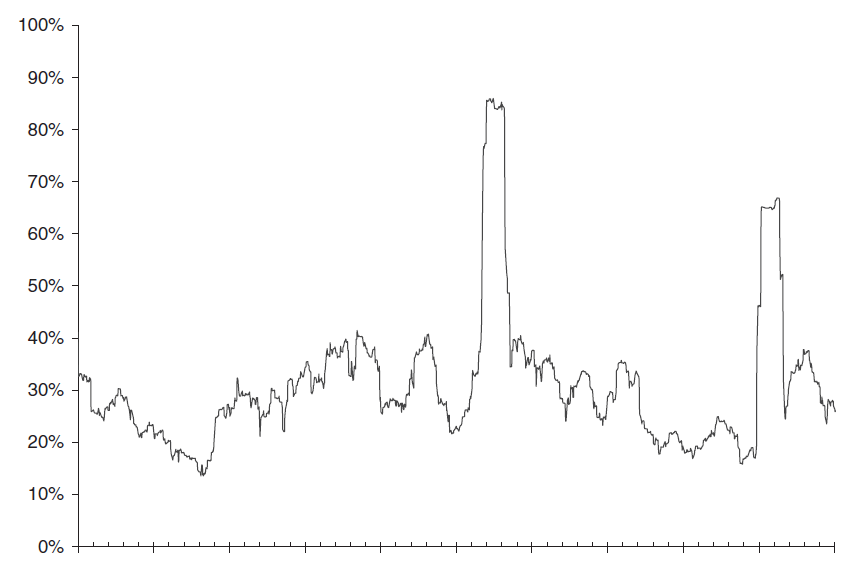
\includegraphics[width=\textwidth]{figure/mw_volatility.png}
        \caption{Moving-window volatility}
    \end{subfigure}
    \begin{subfigure}[b]{0.4\textwidth}
        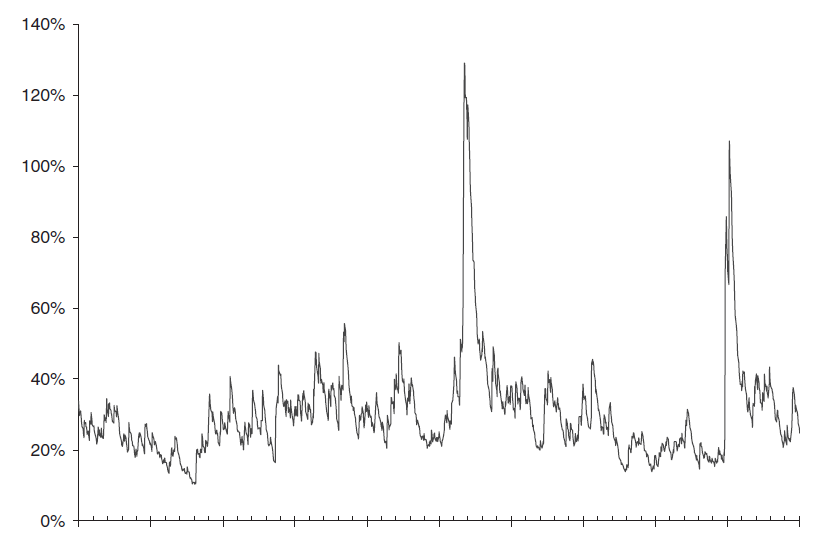
\includegraphics[width=\textwidth]{figure/ew_volatility.png}
        \caption{Exponentially weighted volatility}
    \end{subfigure}
    \caption{Volatility modelling with move-window and exponentially weighted average}
    \label{fig:volatility_modelling_00}
\end{figure}

Figure \ref{fig:volatility_modelling_00} uses the same stock price to estimate the volatility following the moving-window technique and the exponentially-weighted moving average technique. It is clear shown that the first has plateauing whereas the second doesn't have.


\subsubsection{A simple GRACH model}
Put the preceeding models together to get:
\begin{equation}
	\sigma_n^2 = \alpha \bar{\sigma}^2 + (1 - \alpha) \left( \lambda \sigma_{n-1}^2 + (1 - \lambda) R_n^2 \right)
\end{equation}
This is \textbf{GARCH} model, for \textbf{Generalized Autoregressive Conditional Heteroscedasticity}.


\subsubsection{Range-based estimation of volatility}
The problem with estimating volatility is that you need lots and lots of data to avoid sampling-error problems. But then if you use too many days worth of data you will be trying to estimate a parameter during a period when that parameter is almost certainly varying. To avoid this problem, one can use more information contained within a single day which is going down to finer timescales for the data. The problem with that is the behavior of returns over very short timescales, such as minutes, does not appear to be Normally distributed. There is even some evidence that the returns do not have a finite standard deviation. Setting aside such worries, for now. 


\paragraph{Traditional close-to-close measure}
When the drift is small:
\begin{equation}
	\sigma_{cc}^2 = \frac{1}{n} \sum_{i=1}^n \left( \log \left( \frac{C_i}{C_{i-1}} \right) \right)^2
\end{equation}
Here there is a slight change of notation from before; $C_i$ is the closing price on the $i$-th day. To adjust this for the drift take:
\begin{equation}
	\sigma_{cc}^2 = \frac{1}{n-1} \sum_{i=1}^n \left( \left( \log \left( \frac{C_i}{C_{i-1}} \right) \right)^2 - \frac{\left( \log \left( \frac{C_n}{C_0} \right) \right)^2}{n(n-1)} \right)
\end{equation}


\paragraph{Parkinson 1980}
This estimator uses extreme value, the highs $H$ and the lows $L$ during the day:
\begin{equation}
	\sigma_{p}^2 = \frac{1}{4n \log(2)} \sum_{i=1}^n \left( \log \left( \frac{H_i}{L_i} \right) \right)^2
\end{equation}
This is five times more efficient than the close-to-close estimate which means for the same amount of data the variance of the data is one fifth that of the close-to-close measure.


\paragraph{Garman \& Klass 1980}
At 7.4 times more efficient than close-to-close, we have:
\begin{equation}
	\sigma_{gk}^2 = \frac{1}{n} \sum_{i=1}^n \left( 0.511 \left( \log \left( \frac{H_i}{L_i} \right) \right)^2 - 0.019 \log \left( \frac{C_i}{O_i} \right) \log \left( \frac{H_i L_i}{O_i^2} \right) - 2 \log \left( \frac{H_i}{O_i} \right) \log \left( \frac{L_i}{O_i} \right) \right)
\end{equation}
Here $O_i$ is the opening price.


\paragraph{Rogers \& Satchell 1991}
Parkinson and Garman \& Klass are not independent of the drift. Our last simple volatility estimation is:
\begin{equation}
	\sigma_{rs}^2 = \frac{1}{n} \sum_{i=1}^n \left( \log \left( \frac{H_i}{C_i} \right) \log \left( \frac{H_i}{O_i} \right) + \log \left( \frac{L_i}{C_i} \right) \log \left( \frac{L_i}{O_i} \right) \right)
\end{equation}



\section{FDM solutions for Black-Scholes equation (one-factor model)}
\cite{platen_numericalsde_1977, gm_numericalsde_1994, dh_introsde_2001, hg_sdematlab_2006, sm_introsde_2010, mb_numericalsde_2018}

\subsection{Introduction}
Not yet...



\subsection{Differentiation using the grid}
Not yet...



\subsection{Approximating Greeks}
Not yet...



\subsection{Boundary conditions and payoffs}
Not yet...



\subsection{Explicit method}

\subsubsection{Black-Scholes equation}
Not yet...


\subsubsection{Convergence}
Not yet...


\subsubsection{European option}
Not yet...


\subsubsection{American option}
Not yet...


\subsubsection{Runge-Kutta method}
Not yet...


\subsection{Implicit method}

\subsubsection{Crank-Nicolson method}
Not yet...



